\subsection{DP0.2 - processing} \label{sec:dp0.2}

The Milestone L2-DP-0040 includes re processing on IDF of the data set previously served as part of L2-DP-0020.
This requires a workflow system and associated tools to preferably make this quite automated.
Demonstrating a portable set of cloud enabled tools based on Butler Gen3 and PanDA would help to allay the main risk of moving to a new Data Facility in operations.
As of today, processing based on Butler Gen3 has been limited to a very small scale, and no scalability testing has been performed. For L2-DP-0040 we intend to reprocess DC2 RC6  dataset late in 2021 or early 2022.

\subsubsection {Purpose of DP0.2}
The purpose of DP0.2 is manifold, in order of priority:
\begin{enumerate}
	\item generate a fully self-consistent data release for the scientists to publish papers on
	\item Is the purpose to follow a formal data release process with backporting and CCB approvals before allowing new software versions to be used but still taking into account that construction is still ongoing and some flexibility is warranted
	\item perform mini runs early on to improve the chosen pipeline release

	\item Serve as an operations rehearsal for DRP.
\end{enumerate}


\subsubsection {Policy committee} \label{sec:policy}

There are certain decisions which will need to be made are best handled in a smaller forum than DPLT.
This may include:

\begin{itemize}
\item Campaign polices
\item Version of pipelines to use and patches which are needed
\item Version of QA tooling which needs to run (and where/how to run it)
\item Other operational considerations
\end{itemize}

Such decisions will be endorsed by DPLT but advised by a smaller committee more connected to the issues.
The members will be the following (or their delegated representative):

\begin{itemize}
\item Hsin-Fang Chiang
\item Tim Jenness
\item Yusra AlSayyad
\item Colin Slater
\end{itemize}

This is basically  one representative each from Science Pipelines, V\&V, Middleware, and Execution.
It also serves as a trial for operations proper.

\subsubsection {Science pipelines release} \label{sec:release}
We have milestone L3-AP-0010  for the DP0.2 release which is satisfied by v22.0.1 of the science pipelines. This will be good to evaluate PanDA.
For the actual reprocessing, given the timeline, we will make a v23 release when we have the weekly in a state we feel os good for DP0.2.
Should that need fixes they will then be incremental patches on v23.

Hence the delivery of v23  will be driven by the need for DP0.2 rather than time based - this is a more operational way to approach the release.
It will also require support of this releases version for a period of time. This implies backporting agreed fixes (through RFC to DMCCB). A support period of one year seems reasonable.

\subsubsection {High level workflow of workflows}
Despite that the processing workflow is expressed by a "quantum graph" in the Gen3 middleware, it is not feasible to generate the entire DP0.2 processing workflow in one quantum graph.
Splitting the DP0.2 workflow into multiple BPS submissions is necessary with the current software.
There are different ways to constitute the grouping; the two main options are to manage by sky location and to manage by pipeline step.
Each step is a subset of pipelines as in the pipeline definition file\footnote{\url{https://github.com/lsst/obs_lsst/blob/master/pipelines/imsim/DRP.yaml}}.
For DP0.2 processing, we will manage by step and sequence points will be introduced between the steps.
This is not strictly necessary for the DC2 data, but it is the expected mode of processing the actual Rubin data in the future.

All calibration data will exist in the butler repository before any step starts.
The processing steps and the grouping will be the following:
\begin{enumerate}
  \item \texttt{step1}: isr, characterizeImage, calibrate, writeSourceTable, and transformSourceTable. Processing in this step is independent per detector. We plan to separate all visits into groups and generate one quantum graph (and hence one BPS submission) per visit group. Each quantum graph should have a reasonable size.
\texttt{tract} constraints should not appear in the data query.
  \item Between \texttt{step1} and \texttt{step2}, iterations may be done to fix detector failures using code patch.
  \item \texttt{step2}: consolidateSourceTable, consolidateVisitSummary, makeCcdVisitTable, and makeVisitTable. Processing in this step is independent per visit. Either the same grouping as in \texttt{step1} or a larger grouping with more visits per quantum graph will be used.
  \item \texttt{step3}: coaddition, multiband, object table generation, and other tract-based tasks. Processing in this step is independent per tract. Multiple tracts can be combined and processed together in one quantum graph.
  \item \texttt{step4}: image differencing, forcedPhotCcd, forcedPhotDiffim, and transformDiaSourceCat. Processing in this step is independent per detector. Groups of visits as in \texttt{step1} will be used.
  \item \texttt{step5}: drpAssociation, drpDiaCalculation, and other per-tract forced photometry tasks.
Processing in this step is independent per tract.
Final per-tract grouping.
Same tract grouping as in \texttt{step3} will be used.
  \item Between \texttt{step4} and \texttt{step6}, iterations may be done to fix detector failures using code patch.
  \item \texttt{step6}: consolidateDiaSourceTable. Final per-visit grouping. Groups of visits as in \texttt{step2} will be used.
  \item \texttt{step7}: an afterburner that aggregates all tracts into one global file and make a global per-survey property map.
This depends only on the products from \texttt{healSparsePropertyMaps} in \texttt{step3} and can be run after \texttt{step3} is done.
\end{enumerate}

What tasks each step includes may change until the v23 stack release and is updated in the \texttt{obs\_lsst} package of the software stack (\url{https://github.com/lsst/obs_lsst/blob/master/pipelines/imsim/DRP.yaml}).
However, the number of steps and the grouping (visit-based or tract-based) will be frozen in an earlier milestone before v23 release.

\figref{fig:highLevelWorkflow} illustrates the high level concept and the dependency between individual submissions.

\begin{figure}
\begin{center}
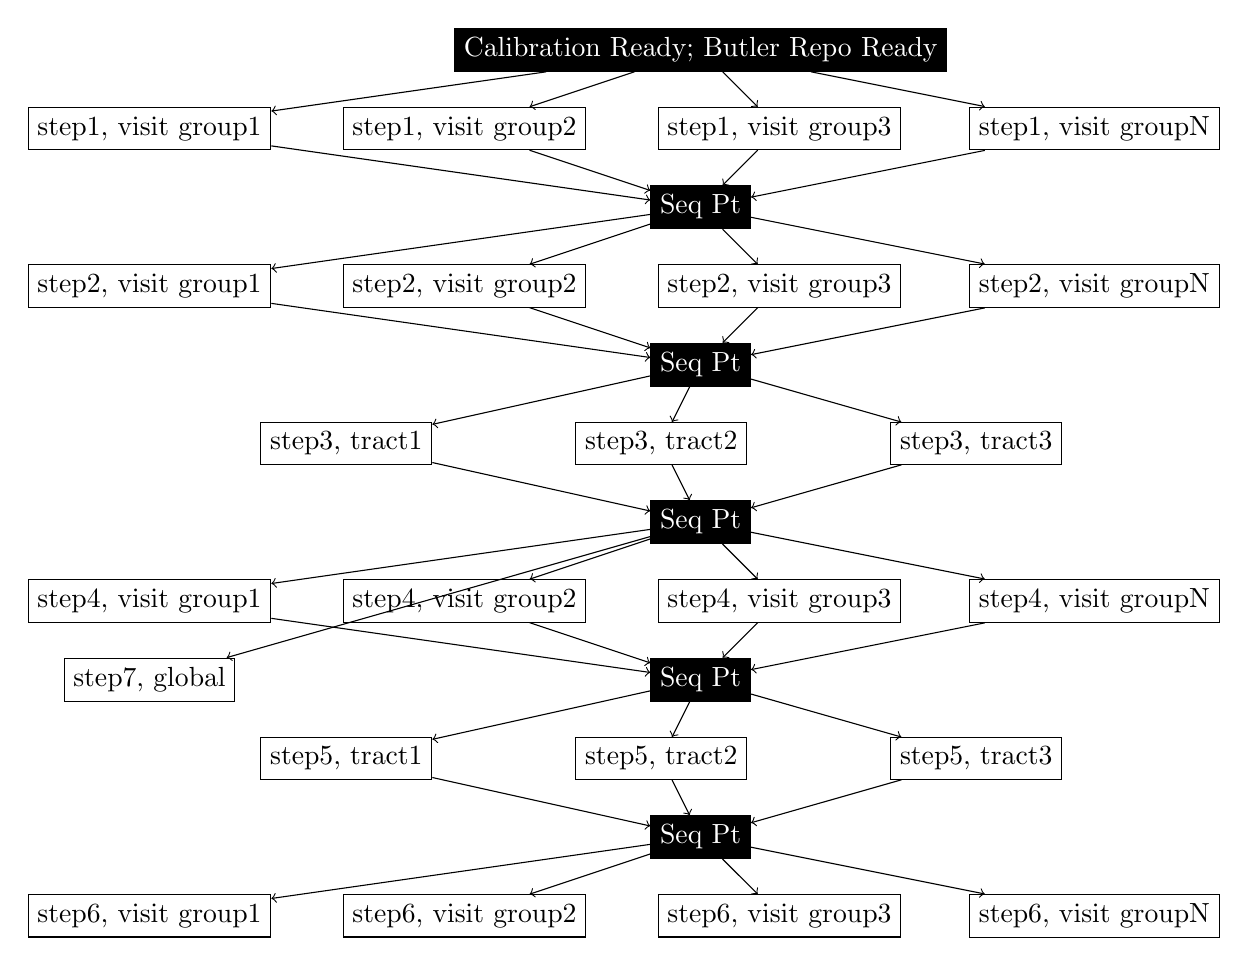
\begin{tikzpicture}[->]
  \node[draw,fill=black,text=white] (step0) at (10,10) {Calibration Ready; Butler Repo Ready};

  \node[draw] (step1v1) at (3,9) {step1, visit group1};
  \node[draw] (step1v2) at (7,9) {step1, visit group2};
  \node[draw] (step1v3) at (11,9) {step1, visit group3};
  \node[draw] (step1v4) at (15,9) {step1, visit groupN};
  \foreach \to in {step1v1,step1v2,step1v3,step1v4}
    \draw (step0) -- (\to);

  \node[draw,fill=black,text=white] (sq1) at (10,8) {Seq Pt};
  \foreach \from in {step1v1,step1v2,step1v3,step1v4}
    \draw (\from) -- (sq1);

  \node[draw] (step2v1) at (3,7) {step2, visit group1};
  \node[draw] (step2v2) at (7,7) {step2, visit group2};
  \node[draw] (step2v3) at (11,7) {step2, visit group3};
  \node[draw] (step2v4) at (15,7) {step2, visit groupN};
  \foreach \to in {step2v1,step2v2,step2v3,step2v4}
    \draw (sq1) -- (\to);

  \node[draw,fill=black,text=white] (sq2) at (10,6) {Seq Pt};
  \foreach \from in {step2v1,step2v2,step2v3,step2v4}
    \draw (\from) -- (sq2);

  \node[draw] (step3v1) at (5.5,5) {step3, tract1};
  \node[draw] (step3v2) at (9.5,5) {step3, tract2};
  \node[draw] (step3v3) at (13.5,5) {step3, tract3};
  \foreach \to in {step3v1,step3v2,step3v3}
    \draw (sq2) -- (\to);

  \node[draw,fill=black,text=white] (sq3) at (10,4) {Seq Pt};
  \foreach \from in {step3v1,step3v2,step3v3}
    \draw (\from) -- (sq3);

  \node[draw] (step4v1) at (3,3) {step4, visit group1};
  \node[draw] (step4v2) at (7,3) {step4, visit group2};
  \node[draw] (step4v3) at (11,3) {step4, visit group3};
  \node[draw] (step4v4) at (15,3) {step4, visit groupN};
  \foreach \to in {step4v1,step4v2,step4v3,step4v4}
    \draw (sq3) -- (\to);

  \node[draw,fill=black,text=white] (sq4) at (10,2) {Seq Pt};
  \foreach \from in {step4v1,step4v2,step4v3,step4v4}
    \draw (\from) -- (sq4);

  \node[draw] (step7) at (3, 2) {step7, global};
  \draw (sq3) -- (step7);

  \node[draw] (step5v1) at (5.5,1) {step5, tract1};
  \node[draw] (step5v2) at (9.5,1) {step5, tract2};
  \node[draw] (step5v3) at (13.5,1) {step5, tract3};
  \foreach \to in {step5v1,step5v2,step5v3}
    \draw (sq4) -- (\to);

  \node[draw,fill=black,text=white] (sq5) at (10,0) {Seq Pt};
  \foreach \from in {step5v1,step5v2,step5v3}
    \draw (\from) -- (sq5);

  \node[draw] (step6v1) at (3,-1) {step6, visit group1};
  \node[draw] (step6v2) at (7,-1) {step6, visit group2};
  \node[draw] (step6v3) at (11,-1) {step6, visit group3};
  \node[draw] (step6v4) at (15,-1) {step6, visit groupN};
  \foreach \to in {step6v1,step6v2,step6v3,step6v4}
    \draw (sq5) -- (\to);

\end{tikzpicture}

\end{center}
\caption{Illustration of the high level DRP workflow for DP0.2. Each white box represents a BPS submission which is a workflow on its own. Typically each submission runs a quantum graph of tens of thousands quanta.
\label{fig:highLevelWorkflow}}
\end{figure}

Discussions:
\begin{enumerate}
  \item Will DP0.2 run calibration product production and generate new master calibration data? No, existing calibration data from DP0.1's repo will be used.
  \item Should \texttt{analysis\_drp} be included? Probably yes and it will be added into one of the existing steps before the freeze date.
  \item Should \texttt{faro} be included? Probably yes. \texttt{faro} tasks should be combined into the existing DRP steps in the pipeline definitions and no extra step is expected from \texttt{faro}. They will be added before the freeze date.
  \item The afterburner task in \texttt{step7} is not written yet but will be added as a proper Gen3 pipetask before the freeze date.
  \item Non-Gen3 tasks such as \texttt{pipe\_analysis}, \texttt{qa\_explorer}, \texttt{validate\_drp}, \texttt{verify}, etc. will not be included in DP0.2 production.
  \item Is there any other analysis pipeline that needs to be run? The assumption is no.
  \item Is there anything else that needs to be run and not included in the "steps"? The assumption is no.
\end{enumerate}

Caveats:
\begin{enumerate}
  \item Doing the production per step and introducing sequence points between steps may lead to longer processing time in calendar days, mostly due to the additional manual intervention needed. Longer timeline should be planned.
  \item Data products in the DP0.2 data release will likely be generated by more than one single version of the Rubin \texttt{lsst\_distrib} software stack. Incremental patches may be used in later steps, or even different patches may be used for different data within one step.
\end{enumerate}

\subsection {Workflow engine}
BNL have been working to demonstrate PanDA with Gen3 for a while. July 2021 is a decision point on using this for DP0.2
\citeds{RTN-013} provided the goals for this task. \citeds{DMTN-168} provides guidelines on how to use this system.


\subsection {Catalogs}
In DP0.2, Science Pipelines reprocessed outputs include a number of catalogs
as parquet data products.
The parquet tables will be accessible as Butler datasets along with other DP0.2 data products, and their contents will be ingested in Qserv and made availble through TAP.
The Butler dataset names of these tables are the following:
\begin{enumerate}
  \item \texttt{objectTable\_tract}
  \item \texttt{sourceTable\_visit}
  \item \texttt{forcedSourceTable}
  \item \texttt{diaObjectTable\_tract}
  \item \texttt{diaSourceTable\_tract}
  \item \texttt{forcedSourceOnDiaObjectTable\_tract}
\end{enumerate}

There will also be parquet data products \texttt{visitTable} and \texttt{ccdVisitTable} in the Butler repo, but it is not decided yet whether they will be ingested in Qserv and made availble through TAP.

All five tables from DP0.1 will be retained and made available in DP0.2
(the \texttt{dp01\_dc2\_catalogs} database; \secref{sec:dp01products}).
